Travel and tourism industry contributed around 7.61 trillion USD to world global economy in 2016\footnote{https://www.statista.com/topics/962/global-tourism/}\footnote{http://www.hospitalitynet.org/news/4069673.html} and it is steadily growing field with big potential. According to a BBC article published in 2013\footnote{http://www.bbc.co.uk/schools/gcsebitesize/geography\newline/tourism/tourism\_trends\_rev2.shtml} the main reasons of tourism growth are: more affluence, greater awareness, more leisure time and more choice. These features are mostly mentioned in connection to more industrialized and wealthy continents as Europe or North America, but it last year, other continents and counties are decreasing the difference which opens the tourism market even more.

As we can see in the figure \ref{fig:touristsPerYear} there are many people who are travelling because of tourism, but compare to the total number of people on the Earth there are more who cannot travel and it can be due to several reasons. The biggest one would definitely be lack of money, for instance, in 2013 still 14.5\% of all Americans, lived below the poverty line. We do not think that a single technology improvement can solve this problem and it is also not the point of this paper. We would like to focus on people who cannot travel because lack of time, mobility problems or age.

According to Darcy and Dickson\cite{darcy2009whole} up to 30\% of a population will have higher access requirements at any point in time during their lives which can affect their ability to travel. This percentage does not cover only missing limbs, but also requirements of some elder to visit their doctors frequently of dependency on medicament. We believe, people with some limitations deserve to get back the feeling of equality and gain back their dignity. We feel it is important to open the gates of the world to as many people as possible, so people can open their eyes and start care about out blue plane even more. 

There is also another aspect which significantly influences current world tourism - Security and terrorism - as was studied at \cite{bac2015terrorism}. According to this study tourism industry has not fully recover after the incident in 2001 and with the reason that people did not gain their full trust to security system. But, unfortunately, there is no study, how many people would travel more if it would be a danger-free

The most real-experience solution for remote virtual tourism would be a humanoid robot controlled by Virtuix Ommi system\footnote{http://www.virtuix.com/product/omni-package/}. Unfortunately, required robot technology does not exist and even if it would, price of needed technology cause that it would be only for the rich people. Another fact is that, this would not make traveling easier for the people, we would like to focus on. Virtuix system relies on full movement of your body and cannot be controlled by people who have mobility problems and have a problem with real travelling.

We are experiencing rapid technology development of drone and virtual reality technology. In the last years, several companies introduced how innovations can be used in industry and services. For instance, Amazon was to use drones for delivering\footnote{http://money.cnn.com/2017/02/14/technology/amazon-drone-patent/} and VR is used for surgery practising\cite{nagendran2013virtual} or pilot training\cite{grabowski2015virtual}, but the main usage of drones and virtual reality is in entertainment. We would like to suggest less costly solution for visiting of remote places via remotely controlled drone with VR system.

Problematic of VR and drone technology has been solved on its own, but combining these technologies bring a lot of difficulties. Current industry drones are controlled by a joystick controller, which according to \cite{mangina2016drones} may allow you maximum control, but learning curve is not sufficient for not frequent users.The paper suggests controlling headset, which is more intuitive (figure \ref{fig:OculusRiftSensorSetup}) and can also be enriched by VR extension. 

Another problem which is also studied at \cite{mangina2016drones} is controlling of remote object which distance from the person who is driving it is changing. It may cause changes in response time of controlled device, in our case drone, and this latency problem can also appear with controlling over an internet connection. This overall problem is also well described and studied at \cite{benjamin2013drone}.

The goal of this paper is to suggest a technical solution which would allow people with any mobility or mental problems to share traveling experience of their relatives and friend. We would like to show, how it is possible to provide at least similar experience of traveling thanks to modern technology with maximum interaction with real surrounding world and freedom to move. Another important aspect is that such solution should not be expensive, so it is affordable for maximum community.

\begin{figure}[t]
    \centering
    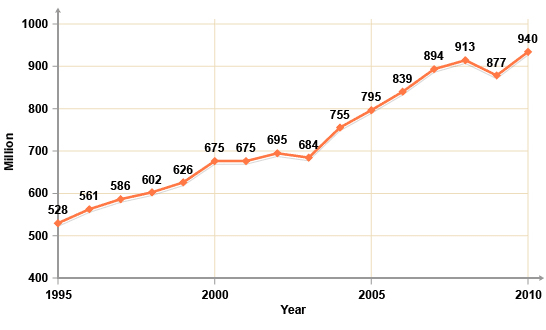
\includegraphics[width=0.40\textwidth]{img/worldTouristsPerYear}
    \caption[Number of tourists per year between 1995 and 2010]{Number of tourists per year between 1995 and 2010\footnotemark}
    \label{fig:touristsPerYear}
\end{figure}
\footnotetext{\url{http://www.bbc.co.uk/schools/gcsebitesize/geography/tourism/tourism\_trends\_rev1.shtml}}

\begin{figure}[t]
    \centering
    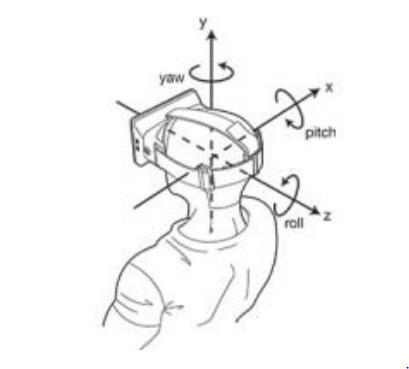
\includegraphics[width=0.40\textwidth]{img/OculusRiftSensorSetup}
    \caption[Oculus Rift Sensor Setup]{Oculus Rift Sensor Setup}
    \label{fig:OculusRiftSensorSetup}
\end{figure}




